\section{Final design}
In \autoref{sec:prototypes-design} we introduced some of our prototypes.
In this section we will show and discuss the final design of some of the front end pages as well as compare some of them to the prototypes we showed in \autoref{sec:prototypes-design}.
\begin{figure}
    \centering
    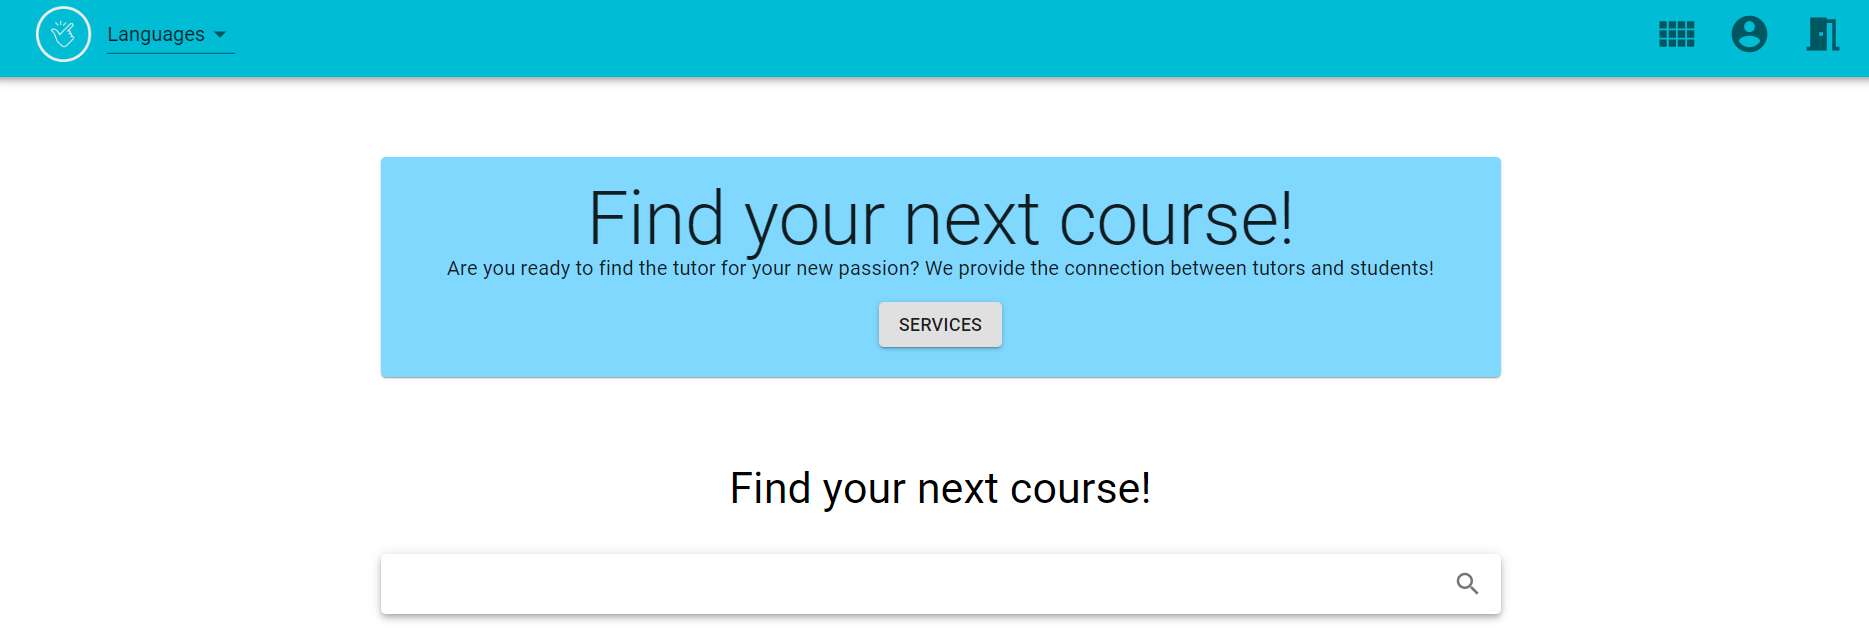
\includegraphics[scale=0.3]{prototypes/landingpageupper.png} 
    \caption{The upper part of the implemented landing page}
    \label{fig:landing-page-upper}
\end{figure}
\begin{figure}
    \centering
    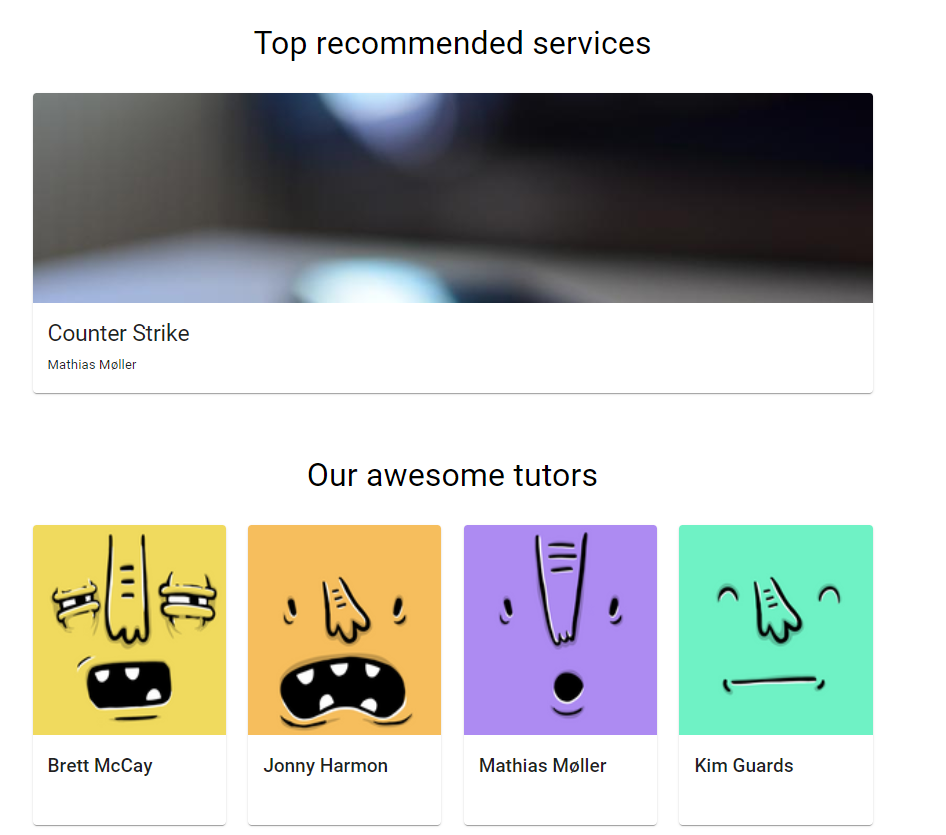
\includegraphics[scale=0.3]{prototypes/landingpagelower.png} 
    \caption{The lower part of the implemented landing page}
    \label{fig:landing-page-lower}
\end{figure}
In \autoref{fig:landing-page} we showed how the prototype for the landing page looked.
The implemented version of the landing page, shown in \autoref{fig:landing-page-upper} and \autoref{fig:landing-page-lower}, ended up looking a bit different.
The layout of the prototype and the implemented version is somewhat the same. 
The same functionality is there, where some of the tutors are shown and the user is able to search for a course. 
\\\\
A new addition in the implemented version is the recommended services that show a couple of services that the current user might be interested in. 
If the user is not logged in, the top rated services are shown instead. 
The implemented landing page is a bit less bloated with information as well and the design is simpler.
\\\\
\begin{figure}
    \centering
    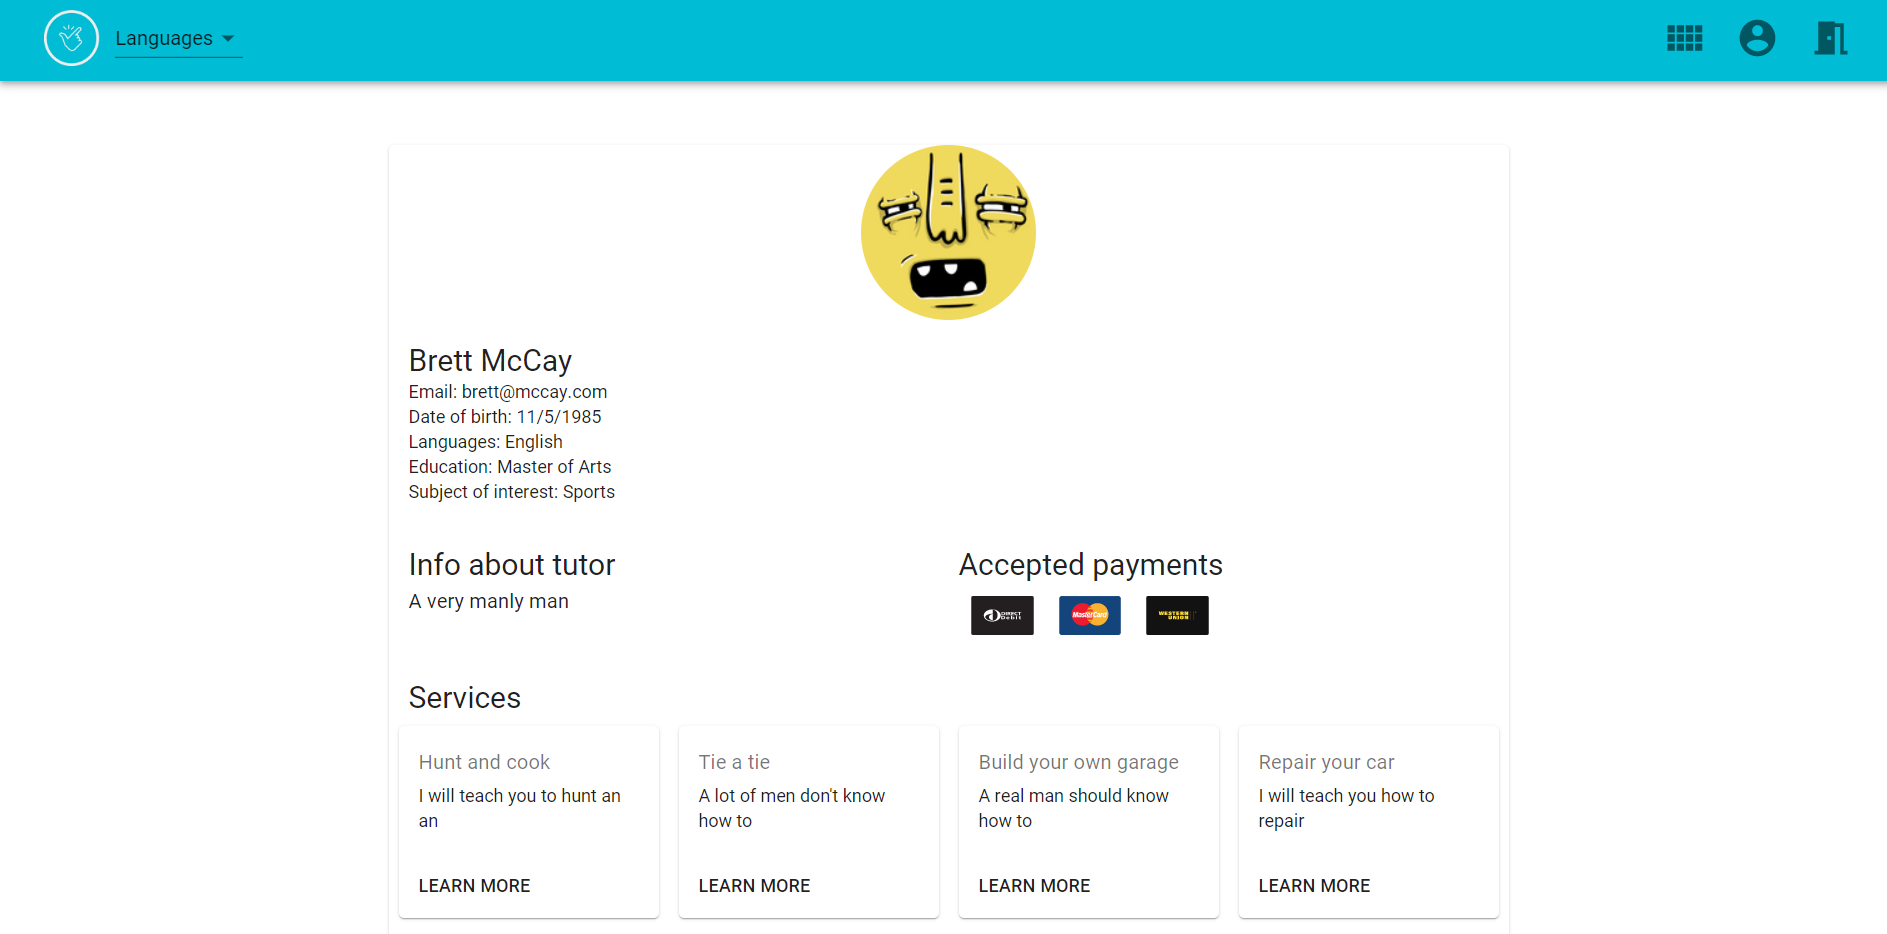
\includegraphics[scale=0.3]{prototypes/tutorinfoimplemented.png} 
    \caption{The implemented view of the tutor information page}
    \label{fig:tutor-info-implemented}
\end{figure}
In \autoref{fig:view-information-on-tutor} we showed the prototype for viewing the information on a tutor.
Because of time limitation and changes in priority during the project, some of the features available on the prototype were not implemented.
The page shows all the basic information about a tutor and it also shows the services that the tutor provides.
Since tutor materials and the calendar were not implemented, it did not make sense to render available material and appointments on the tutor's page.
\begin{figure}
    \centering
    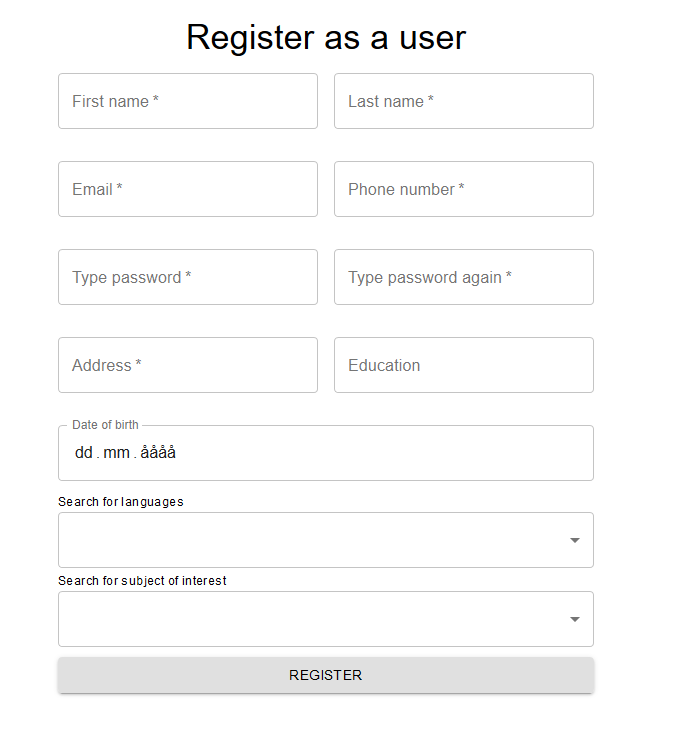
\includegraphics[scale=0.7]{prototypes/registeruser.png} 
    \caption{The page where a new user can be registered in the system}
    \label{fig:register-user-implemented}
\end{figure}
In \autoref{fig:register-user-implemented} the page where a new user can be registered is shown.
This page is pretty much identical to the prototype that we created since we had a good idea from the start of what information a user should be able to fill in. 
We did not show the prototype for this page since there is a standardized way of creating these input forms so there were not any big design decisions to show.
\\\\
\begin{figure}
    \centering
    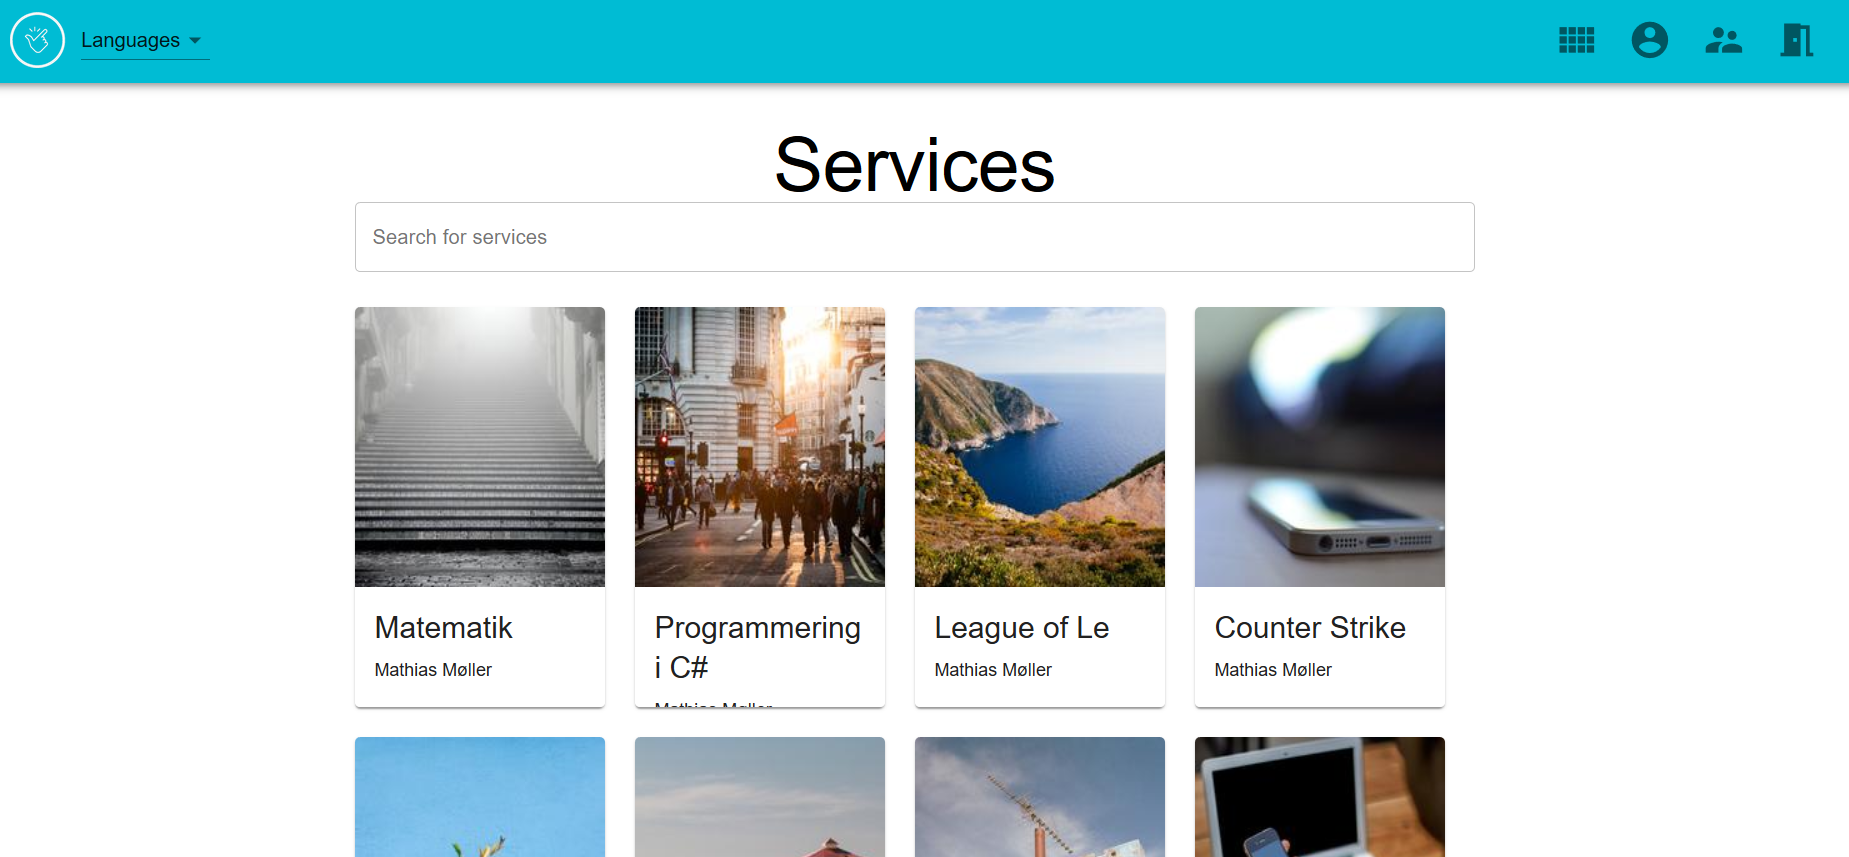
\includegraphics[scale=0.3]{prototypes/services.png}
    \caption{The page where all the services are shown}
    \label{fig:all-services-implemented}
\end{figure}
In \autoref{fig:all-services-implemented} the page that shows all the available services is shown. 
This implementation is pretty much identical to how we envisioned the page would look in our prototypes. 
It should be easier to see what the service is about from the picture and it should be easy to read the title of the service name.
For this reason we made each service card quite large.
We also wanted the user to be able to filter through the services by searching in the search bar. 
The filtering happens as the user is typing so the updates happens instantly.
\\\\
\begin{figure}
    \centering
    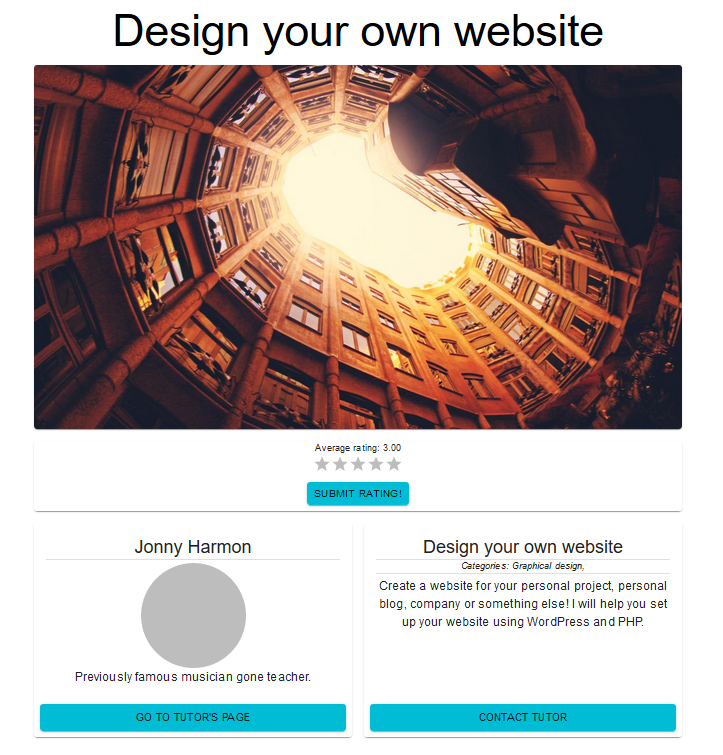
\includegraphics[scale=0.7]{prototypes/showservice.png} 
    \caption{The page that shows details about a service}
    \label{fig:show-service-implemented}
\end{figure}
\autoref{fig:show-service-implemented} shows the page for details of a service.
At the top of the page it should be easy to see the title and picture so the user knows that they are at the correct service.
At the bottom of the page the user can read more details about the service and the tutor that provides the service.
If the user is interested in the service, they can click the contact tutor button to get in contact with the tutor.
The user is also able to rate the service from one to five stars, and an average rating is shown to indicate the level of quality of the service.
